\section{Evaluation}\label{sec:eval}

We developed \( \tool \) as an open-source tool\footnote{The URL of the tool is
anonymized due to a double-blind review process.}, and evaluated the tool
based on the following research questions:
\begin{itemize}[leftmargin=0.5cm]
\item RQ1. \textbf{Coverage:} How much percentage of 
the syntax and semantics does \( \tool \) automatically extract from ES7 to ES10?
\item RQ2. \textbf{Correctness:} Does \( \tool \) extract an IR-based formal
semantics from ECMAScript correctly?
\item RQ3. \textbf{Forward Compatibility:} Is \( \tool \) applicable to language
features ready for inclusion in the next ECMAScript (ES11)?
\end{itemize}


\subsection{Coverage}

\begin{table}[t]
  \caption{Syntax coverage: Number of productions in each specification
and in each update between adjacent versions,
from \textit{all} of which \( \tool \) automatically generated parsers}
  \label{fig:syntax-all-version}
\vspace*{-1em}
\small
  \[
    \begin{array}{c?r|r|r|r?r}
      \textbf{Version}
      & \multicolumn{1}{c|}{\textbf{ES7}}
      & \multicolumn{1}{c|}{\textbf{ES8}}
      & \multicolumn{1}{c|}{\textbf{ES9}}
      & \multicolumn{1}{c?}{\textbf{ES10}}
      & \multicolumn{1}{c}{\textbf{Average}}\\\toprule
      \text{\# Lexical productions}
      & \text{78}
      & \text{78}
      & \text{78}
      & \text{81}
      & \text{78.75}\\\hline
      \text{\# Syntactic productions}
      & \text{157}
      & \text{167}
      & \text{167}
      & \text{174}
      & \text{166.25}\\
    \end{array}
  \]
  \[
    \begin{array}{c?r|r|r?r}
      \textbf{Old version}
      & \multicolumn{1}{c|}{\textbf{ES7}}
      & \multicolumn{1}{c|}{\textbf{ES8}}
      & \multicolumn{1}{c?}{\textbf{ES9}}
      & \multirow{2}{*}{\textbf{Average}}\\\cline{1-4}
      \textbf{New version}
      & \multicolumn{1}{c|}{\textbf{ES8}}
      & \multicolumn{1}{c|}{\textbf{ES9}}
      & \multicolumn{1}{c?}{\textbf{ES10}}
      & \\\toprule
      \Delta \; \text{\# Lexical productions}
      & \text{3}
      & \text{5}
      & \text{6}
      & \text{4.67}\\\hline
      \Delta \; \text{\# Syntactic productions}
      & \text{140}
      & \text{15}
      & \text{8}
      & \text{54.33}\\
    \end{array}
  \]
\end{table}

We evaluated the coverage of \( \tool \) in two respects: syntax
and semantics.  For syntax, we measured how many grammar
productions in specifications \( \tool \) automatically generated
parsers from, and for semantics, we measured how many abstract
algorithm steps in specifications it automatically generated the
JavaScript semantics from.  Because \( \tool \) utilizes common
patterns in the converged writing style since ES7 as we discussed in
Section~\ref{sec:overview}, we evaluated its coverage using the most
recent four versions of ECMAScript, ES7 to ES10.  We measured the
numbers for each ECMAScript version and for each update between
adjacent versions.



For syntax, \( \tool \) automatically generated parsers for \textit{all} the
lexical and syntactic productions.  As Table~\ref{fig:syntax-all-version} shows,
the average numbers of lexical and syntactic productions are 78.75 and
166.25, respectively.  Also, the average numbers of annually updated
lexical and syntactic productions between adjacent versions are 4.67 and
54.33, respectively.

\begin{figure}[t]
  \centering
  \begin{subfigure}{0.48\textwidth}
    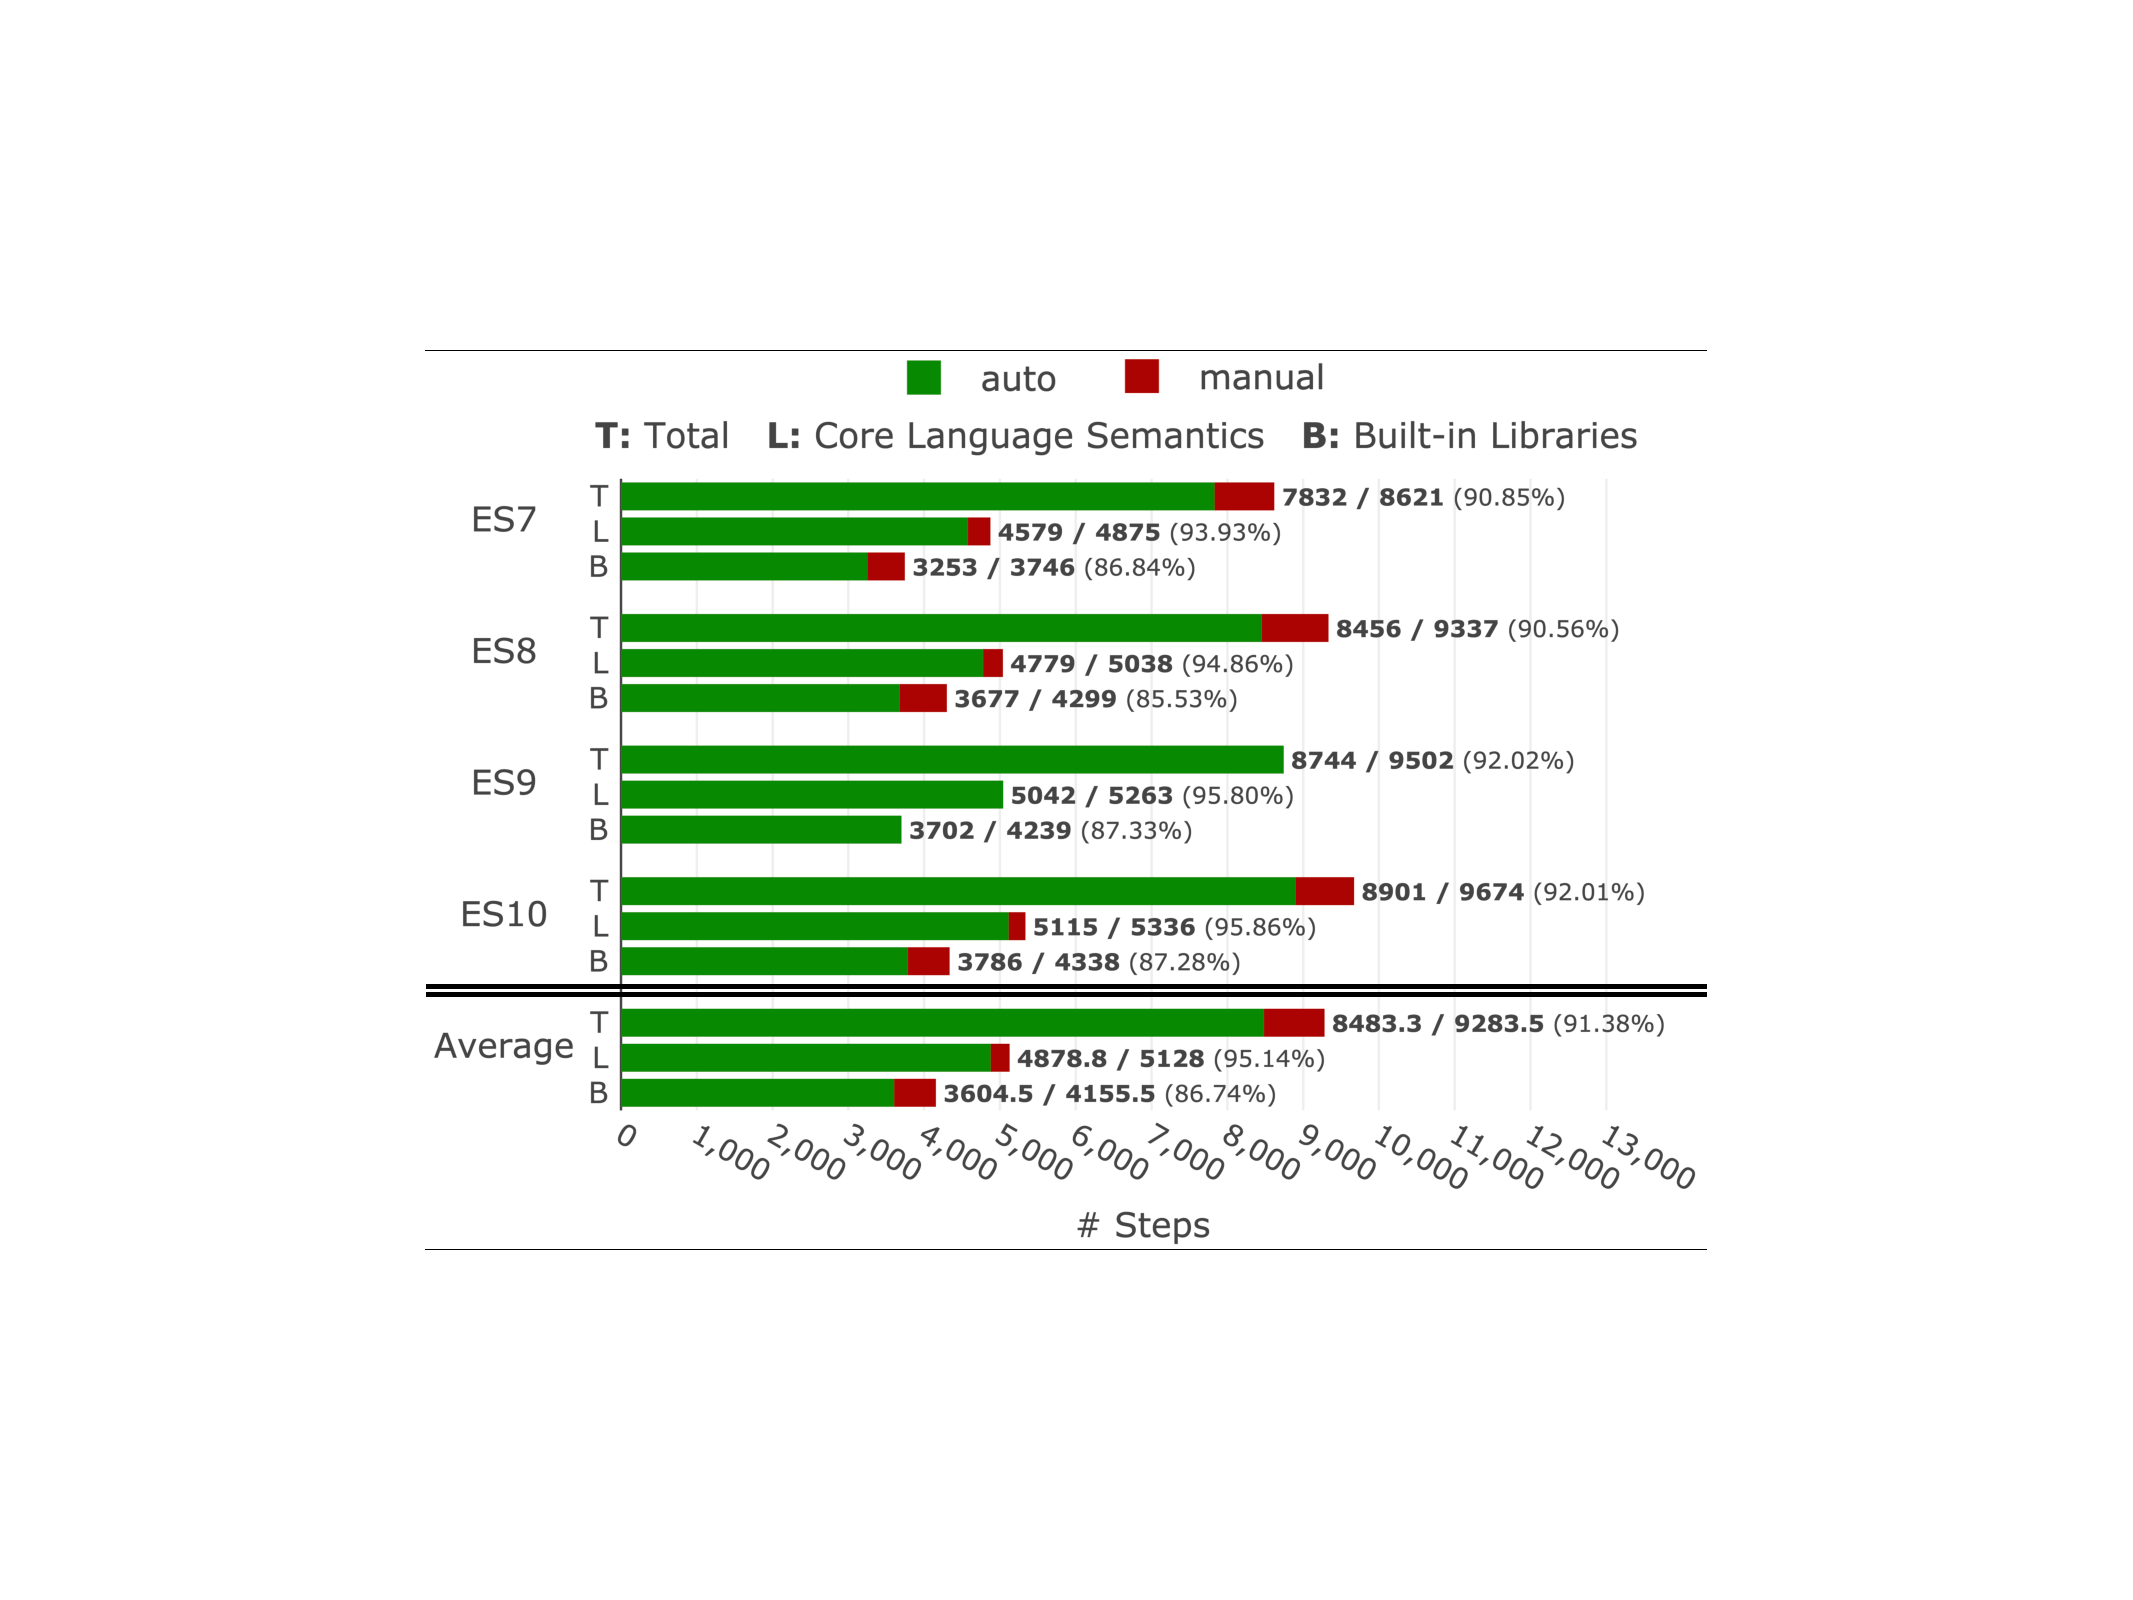
\includegraphics[width=\textwidth]{img/sem-all.pdf}
    \caption{For each ECMAScript version from ES7 to ES10}
    \label{fig:semantics-all-version}
  \end{subfigure}
  \hfill
  \begin{subfigure}{0.48\textwidth}
    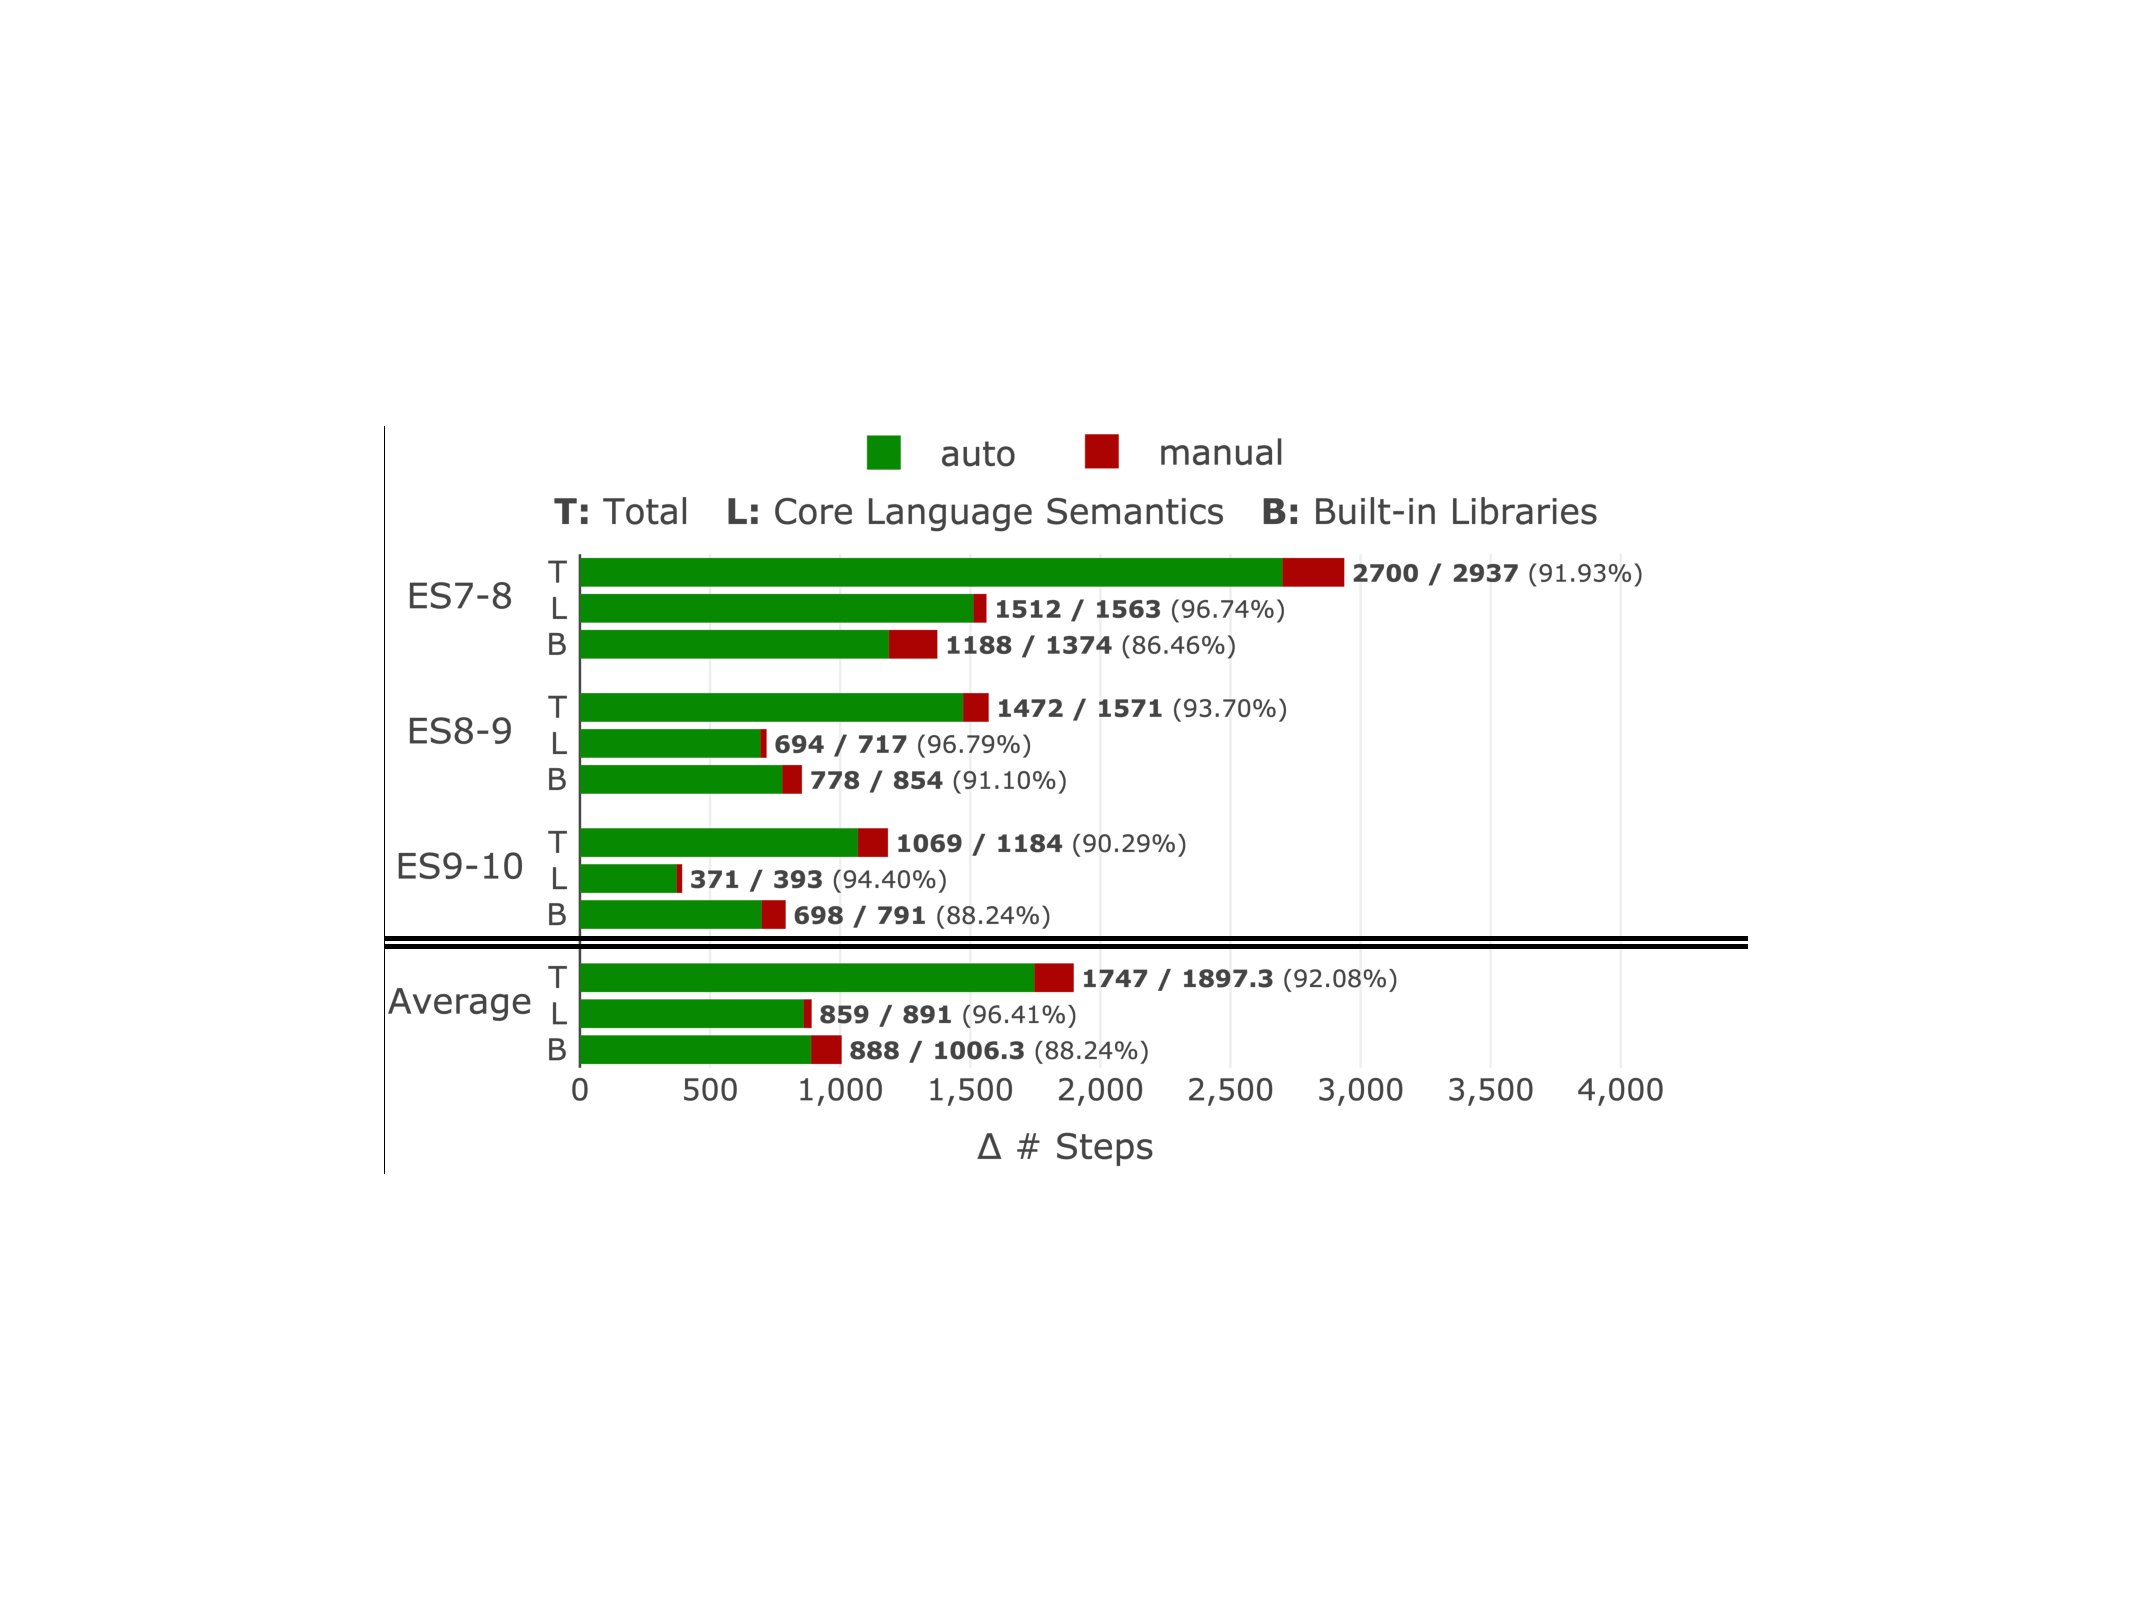
\includegraphics[width=\textwidth]{img/sem-update.pdf}
    \caption{For each update between adjacent versions}
    \label{fig:semantics-all-version-update}
  \end{subfigure}
\vspace*{-.5em}
\caption{Semantics coverage: Number of algorithm steps in specifications,
from which \( \tool \) generated the semantics}
  \label{fig:all-version}
\vspace*{-1.5em}
\end{figure}

For semantics, Figure~\ref{fig:all-version} shows that \( \tool \) automatically
compiled algorithm steps to corresponding \( \ires \) instructions with
the success rate of 95.03\% on average for each ECMAScript version
from ES7 to ES10, and 94.31\% for each update between adjacent
versions.  ECMAScript abstract algorithms describe not only
core language semantics but also built-in libraries with various helper functions.
Note that built-in libraries are written in more diverse styles than
core language semantics due to their own specific functionalities.
Therefore, built-in libraries have lower success rates
(92.55\% for specifications and 91.50\% for updates) than core
language semantics (97.06\% for specifications and 97.14\% for
updates).

Because \( \tool \) automatically extracts the syntax
and semantics from specifications and updates with high coverage rates,
it reduces efforts not only in developing JavaScript tools from scratch
from specifications but also in evolving existing tools for updates.


\subsection{Correctness}\label{sec:check-with-tests}
\begin{table*}[t]
  \centering
  \caption{Specification errors in ES10 and the BigInt proposal ready for
  inclusion in ES11}
  \label{table:spec-errors}
  \vspace*{-.5em}
  \small
  \begin{tabular}{@{}c?c|l|@{}c@{}|c|c|r|@{}r@{}}
\multicolumn{1}{@{}c?}{\bf Name} &
\multicolumn{1}{c}{\bf Feature} &
\multicolumn{1}{c}{\bf Description} &
\multicolumn{1}{@{}c@{}}{\bf Known} &
\multicolumn{1}{c}{\bf Created} &
\multicolumn{1}{c}{\bf Resolved} &
\multicolumn{1}{c}{\bf Existed} &
\multicolumn{1}{@{}c@{}}{\bf \# Fails} \\\toprule
&&&&&&&\\[-1.5em]
    ES10-1 &
    Iteration &
    \makecell[l]{Missing the \code{async-iterate} case in the assertion of\\
 {\bf ForIn/OfHeadEvaluation}} &
    \textsf{X} &
    2018-02-16 &
    2020-03-25 &
    768 days &
    1,116 \\\hline

    ES10-2 &
    Condition &
    \makecell[l]{Ambiguous grammar production for the dangling \code{else} problem in\\
    {\it IfStatement}} &
    \textsf{X} &
    2015-06-01 &
    TBD &
    \multicolumn{1}{c|}{TBD} &
    1 \\\hline

    ES10-3 &
    String &
    \makecell[l]{Wrong use of the \code{=} operator in {\bf
    StringGetOwnProperty}} &
    \textsf{X} &
    2015-06-01 &
    TBD &
    \multicolumn{1}{c|}{TBD} &
    7 \\\hline

    ES10-4 &
    Completion &
    Unhandling abrupt completion in {\bf Abstract Equality Comparison} &
    \textsf{X} &
    2015-06-01&
    2020-04-28 &
    1,793 days &
    9 \\\hline

    ES10-5 &
    Completion &
    \makecell[l]{Unhandling abrupt completion in {\bf Evaluation} of {\it
    EqualityExpression}} &
    \textsf{O} &
    2015-06-01 &
    2019-05-02 &
    1,431 days &
    2 \\\hline

    ES10-6 &
    Await &
    \makecell[l]{Passing a value of wrong type to the second parameter of\\ {\bf PromiseResolve}} &
    \textsf{O} &
    2019-02-27 &
    2019-04-13 &
    45 days &
    1,294 \\\hline

    ES10-7 &
    Function &
    \makecell[l]{No semantics of {\bf IsFunctionDefinition} for
    \code{function(...)\{...\}}} &
    \textsf{O} &
    2015-10-30 &
    2020-01-18 &
    1,541 days &
    306 \\\hline

    ES10-8 &
    Function &
    \makecell[l]{No semantics of {\bf ExpectedArgumentCount} for the base case
    of\\ {\it FormalParameters}} &
    \textsf{O} &
    2016-11-02 &
    2020-02-20 &
    1,205 days &
    81 \\\hline

    ES10-9 &
    Iteration &
    \makecell[l]{Two semantics of {\bf VarScopedDeclarations} for\\ \code{for
    await(var x of e)\{...\}}} &
    \textsf{O} &
    2018-02-16 &
    2019-10-11 &
    602 days &
    0 \\\hline\hline

    BigInt-1 &
    Expression &
    \makecell[l]{Using the wrong variable \code{oldvalue} instead of
    \code{oldValue} in \\ {\bf Evaluation} of {\it UpdateExpression}} &
    \textsf{X} &
    2019-09-27 &
    2020-04-23 &
    209 days &
    \inred{XX} \\\hline

    BigInt-2 &
    Number &
    \makecell[l]{Using {\bf ToInt32} instead of {\bf ToUint32} in \\ {\bf
    Number::unsignedRightShift}} &
    \textsf{X} &
    2019-09-27 &
    2020-04-23 &
    209 days &
    \inred{XX} \\\hline

    BigInt-3 &
    Number &
    \makecell[l]{Using {\bf ToUint32} instead of {\bf ToInt32} in {\bf
    NumberBitwiseOp}} &
    \textsf{X} &
    2019-09-27 &
    2020-04-23 &
    209 days &
    \inred{XX} \\\hline

    BigInt-4 &
    Number &
    \makecell[l]{Unhandling BigInt values in the {\bf Number} constructor} &
    \textsf{O} &
    2019-09-27 &
    2019-11-19 &
    53 days &
    \inred{XX}
  \end{tabular}
\end{table*}

\begin{table}[t]
  \centering
  \caption{Test results for Test262}
  \label{table:test262}
  \vspace*{-.5em}
  \small
  \begin{tabular}{lr}\toprule
    \belowrulesepcolor{gainsboro}
    \rowcolor{gainsboro} \textbf{All Test262 Tests} & \textbf{35,990}\\
    \aboverulesepcolor{gainsboro}\midrule
    Annexes & 1,060\\\hdashline
    Internationalization & 640\\\hdashline
    In-progress features & 5,338\\\midrule
    \belowrulesepcolor{gainsboro}
    \rowcolor{gainsboro} \textbf{ES10 Tests} & \textbf{28,952}\\
    \aboverulesepcolor{gainsboro}\midrule
    Non-strict mode & 1,150\\\hdashline
    Modules & 918 \\\hdashline
    Early errors before actual execution & 2,288 \\\hdashline
    Inessential built-in objects & 6,532 \\\midrule
    \belowrulesepcolor{gainsboro}
    \rowcolor{gainsboro} \textbf{Applicable Tests} & \textbf{18,064}\\
    \aboverulesepcolor{gainsboro}\midrule
    Passed tests & 16,355 \\\hdashline
    Failed tests & 1,709 \\\bottomrule
  \end{tabular}
  \vspace*{-1em}
\end{table}

To evaluate the correctness of \( \tool \), we checked whether the
extracted semantics from the latest ECMAScript (ES10) passes Test262
as of February 28, 2019, when ES10 was branched out.
To focus on the core language semantics of JavaScript, we completed
only necessary parts missing from the extracted AST-IR translator.
As Figure~\ref{fig:all-version}(a) shows, for the abstract algorithms
in ES10, 9,627 steps out of 10,101 steps are
automatically compiled by \textsf{Algorithm Compiler}.
Among the remaining 474 steps, we manually implemented all
missing steps for the core language semantics (137 steps) and
the essential parts of the built-in libraries (\inred{XX} steps out of
337).  We also manually implemented \textsf{Global Setting}
as described in Section~\ref{sec:compiler-impl} for the core language features.
Note that we do not support minor language features such as the
non-strict mode, modules, early errors before actual execution, and
inessential built-in objects.
Among 35,990 tests in Test262, we filtered out 17,926
tests as summarized in Table~\ref{table:test262}.  To focus on ES10,
we excluded 7,038 tests for annexes, internationalization, and
in-progress features.  We also filted out 10,888 tests that use
minor language features.
Finally, for 18,064 applicable tests, the extracted semantics
failed for 1,709 tests.

We investigated the failed tests and found out that they failed due to
specification errors in ES10.  Using the failed tests, we
discovered nine errors: ES10-1 to ES10-9 in
Table~\ref{table:spec-errors}.  Among them, five errors (ES10-5 to
ES10-9) were previously reported and fixed in the current draft of the
next ECMAScript, and the remaining four errors (ES10-1 to ES10-4) were
never reported before.  All four errors were confirmed by TC39, and
will be fixed in the next ECMAScript, ES11.

The specification error ES10-1 is due to a wrong assertion.
While ES9 introduced the \code{for await} iteration statement with a
new {\it iterationKind} tag, \code{async-iterate}, the
\code{ForIn/OfHeadEvaluation} algorithm missed the
\code{async-iterate} case in an assertion, which caused 1,120
tests failed.  We reported the error and proposed a specification fix
to include  the \code{async-iterate} case, and TC39 accepted it on
March 25, 2020.  Because the error was created on February 16, 2018,
it existed for 768 days.

ES10-2 comes from the well-known dangling \code{else} problem
introduced in ALGOL 60~\cite{dangling-else}.  ES10 describes how to
parse it in prose: the \code{else} statement should be associated with
the nearest \code{if} statement.  Because it is written in prose
rather than in the ES10 grammar productions, it caused one test
failed.  We proposed a fix to revise the ambiguous grammar production,
and TC39 confirmed it on April 23, 2020.

ES10-3 is due to a misuse of the \code{=} operator for numbers.
In abstract algorithms, ``{\it x} = {\it y}'' denotes equality testing
for double-precision 64-bit binary format IEEE 754-2008 values;
thus, \mbox{``+0 = -0''} evaluates to true.  However, to check whether
{\it index} is exactly the same with -0,
{\bf StringGetOwnProperty} used \mbox{``{\it index} = -0''},
which is true even when {\it index} is +0.
It caused seven tests failed.  We proposed a fix, which is
confirmed on April 22, 2020.

ES10-4 and ES10-5 happened because ES10 did not handle
abrupt completion from function calls.  Our proposed fix to ES10-4 was
accepted on April 28, 2020, and ES10-5 was resolved on May 2, 2019
after existing for 1,431 days.

ES10-6 is due to incorrect uses of an abstract algorithm.
While {\bf PromiseResolve(C, x)} expects a JavaScript object for its
second argument, ES10 passed a list of values rather than an object in
three invocations of {\bf PromiseResolve}.  The wrong invocations were
introduced on February 27, 2019 and caused 1,294 tests failed.
They were fixed on April 13, 2019 after existing 45 days.

ES10-7 and ES10-8 happened because ES10 missed semantics for some
cases.  They both existed for more than 1,200 days.

ES10-9 is due to multiple semantics.  While no tests in Test262 fail
with any of the semantics, we could detect this error via {\sf Spec
Extractor} even before executing the semantics. It is supplementary merit of
the mechanization of IR-based semantics extraction.

After resolving the nine specification errors in ES10, we extracted a
semantics from the revised specification.  The extracted semantics
from the revised ES10 passed all 18,064 applicable tests in Test262,
which shows that \( \tool \) extracts an IR-based formal semantics
from ECMAScript correctly.  In addition, the evaluation witnesses that
\( \tool \) can detect specification errors effectively.
We could detect not only five previously-known errors
but also four new errors.  We believe that \( \tool \) bridges gaps
between ECMAScript written in a natural language and executable tests
in Test262.

\begin{table}[t]
  \centering
  \caption{Proposals that will be included in ES11}
  \label{table:spec-prop-result}
  \vspace*{-1em}
  \small
  \begin{tabular}{@{}c@{}?r|@{~}r@{~}|@{}c@{}|@{}c@{}|c@{}}
    \multicolumn{1}{@{}c@{}?}{\multirow{2}{*}{\bf Proposal}} &
    \multicolumn{2}{@{~}c@{~}|}{\bf \( \Delta \) \# Prod.} &
    \multicolumn{1}{@{~}c@{~}|}{\multirow{2}{*}{\bf \( \Delta \)\! \#\! Steps}} &
    \multicolumn{1}{@{~}c@{~}|}{\multirow{2}{*}{\bf \( \Delta \)\! \#\! Tests}} &
    \multicolumn{1}{c@{}}{\multirow{2}{*}{\bf \# Tests}} \\\cline{2-3}

    &
    \multicolumn{1}{@{~}c@{~}|}{\bf Lex.} &
    \multicolumn{1}{@{~}c@{~}|}{\bf Syn.} &
    &\\\toprule

    \code{matchAll} of \code{String} &
    0 &
    0 &
    9/9 &
    5/5 &
    18,064/18,064\\\hline

    \code{import()} &
    0 &
    2 &
    22/23 &
    0/0 &
    18,064/18,064\\\hline

    \code{BigInt} &
    4 &
    0 &
    258/323 &
    \inred{207}/207 &
    \inred{18,064}/18,064\\\hline

    \code{Promise.allSettled } &
    0 &
    0 &
    79/85 &
    50/50 &
    18,064/18,064\\\hline

    \code{globalThis} &
    0 &
    0 &
    1/1 &
    1/1 &
    18,064/18,064\\\hline

    \code{for-in}  mechanics &
    0 &
    0 &
    36/37 &
    0/0 &
    18,064/18,064\\\hline

    Optional Chaining &
    3 &
    3 &
    72/74 &
    19/19 &
    18,064/18,064\\\hline

    Nullish Coalescing Op. &
    1 &
    4 &
    10/10 &
    21/21 &
    18,064/18,064\\\hline

    \code{import.meta} &
    0 &
    2 &
    15/15 &
    0/0 &
    18,064/18,064\\\hline

    {\bf Total} &
    8 &
    11 &
    502/577 &
  \end{tabular}
\vspace*{-1em}
\end{table}

\subsection{Forward Compatibility}
We evaluated whether \( \tool \) is forward compatible by applying it
to the proposals ready for inclusion in ES11.  Because
ECMAScript is an open-source project, various proposals for new
features are available with their own specification changes and tests.
A separate repository~\cite{proposals} maintains them in six
stages: Stage 0 to Stage 3, Finished, and Inactive.  A proposal
starts with Stage 0, and the TC39 committee examines proposals in Stage 3.
If a proposal is confirmed, the committee changes
its stage to Finished and integrates it into the next ECMAScript.
Otherwise, its stage becomes Inactive.

We applied \( \tool \) to all nine Finished proposals as shown in
Table~\ref{table:spec-prop-result}.
Collectively, the proposals modified \inred{XX} lexical and
\inred{XX} syntactic productions, and \( \tool \) successfully
synthesized parsers for them.  The synthesized parsers parse all
applicable tests for all proposals.  For abstract algorithms,
\inred{XXX} steps out of \inred{XXX} are automatically converted to
corresponding \( \ires \) instructions by \textsf{Algorithm Compiler}
without changing {\sf Compile Rules}.  Thus, \( \tool \) has the
success rate of \inred{XX.XX\%} on average for forthcoming proposals.

We checked the extracted semantics from the proposals
by implemented missing parts of the AST-IR translator for
each proposal and checking the semantics with Test262.  All of them
passed all applicable tests except the semantics from the
\code{BigInt} proposal.  It failed for \inred{XX} tests out of 207
applicable tests for the proposal and \inred{XXXX} tests out of
\inred{XXXXX} applicable tests for ES10.

Using the failed tests, we discovered four errors in the
BigInt proposal: three new errors (BigInt-1 to BigInt-3) and one known
error (BigInt-4) as summarized in Table~\ref{table:spec-errors}.
All of them were confirmed by TC39 and will be fixed in ES11.
The proposal added two new types: BigInt as a new type of primitives
and Numeric as a unified type of the original Number type and the new BigInt type.
Therefore, it not only added new algorithms for BigInt but also modified
all existing algorithms for Number values.
The error BigInt-1 is due to a misuse of the variable 
\code{oldValue} in {\bf Evaluation} of {\it UpdateExpression}.
BigInt-2 and BigInt-3 break the backward compatibility because of
misusing {\bf ToInt32} and {\bf ToUint32}
in unsigned right shift operators and bitwise operators, respectively.
BigInt-4 is due to missing BigInt primitives in the Number constructor.
On average, four errors existed for \inred{XXX} days in the proposal.

After fixing the errors in the proposal, we extracted a semantics from
the revised specification.  The extracted semantics passed all 207
applicable tests for the proposal and \inred{XXXXX} applicable tests
for ES10.  Thus, \( \tool \) also correctly extracts an IR-based
semantics from future proposals, which implies that it is forward compatible.
